%=================================================================
\section{Introduction}\label{sec-intro}


Emotion detection has attracted great interest 
in the natural language processing (NLP)
in the last few years.
In sentiment analysis, 
affective states are generally represented 
using either categorical or dimensional approaches.
The most popular categorical approach represents is 
Ekman’s six basic emotions 
(e.g., anger, happiness, fear, sadness, disgust and surprise)
The dimensional approach represents affective states by using
continuous numerical values in two/three dimensions,.
The valence-arousal (VA) dimensions model , 
as shown in ~\Cref{fig:va}. 
The valence represents the degree of 
positive and negative, 
while the arousal represents the degree of 
excitement and calm. 
In 1994,
Bradley and Lang proposed 
Valence- Arousal-Dominance model,
as shown in ~\Cref{fig:vad}.
And Dominance perceived degree of control in a (social) situation.
Based on this representation, 
any affective state can be represented as a point 
in the VA/VAD coordinate plane. 
Based on this representation, 
any affective state can be represented as 
a point in the VA/VAD coordinate plane.

In this paper, 
we want to predict  
multiple emotion dimension scores for an input text.
A new machine learning paradigm called 
Label Distribution Learning (LDL) 
was proposed in recently years.
Similarly,
we propose an dimensional emotion distribution learning (DEDL) algorithm
Different from the previous approaches, 
DEDL assumes that
each sentence contains a mixture of 
dimensional emotions with different intensities. 
We can label each sentence with 
an label distribution vector 
where elements corresponds to 
dimensional emotions and 
the value of each element indicates the intensity of the dimensional emotions. 
We require that each vector element has a value 
between 0 and 1 and they sum up to 1.

Use Dimensional Emotions Distribution Learning
to predict multiple emotion dimension scores for an input text.
Then use the predicted VAD and notational VAD to 
do emotion classification.
Also, 
we will use the Deep Learning to do emotion classifiction.

\begin{figure}[htbp]
	\begin{minipage}[t]{0.5\linewidth}
		\centering
		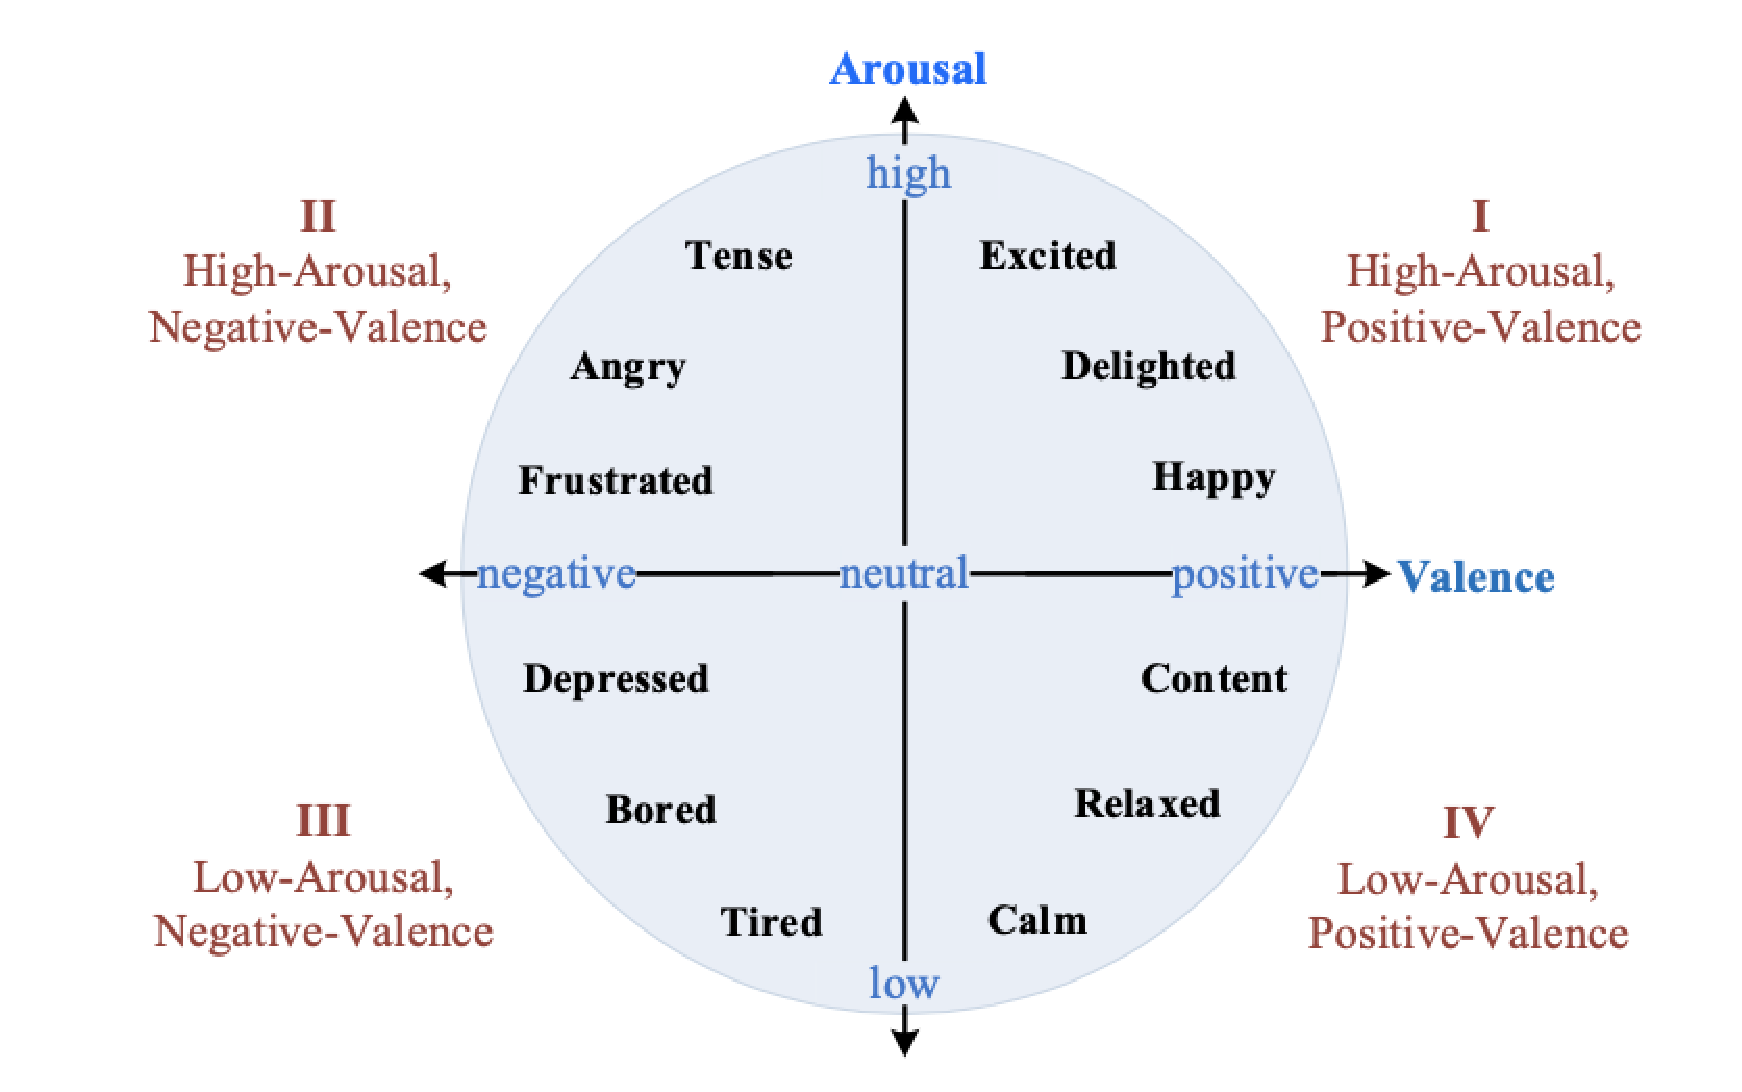
\includegraphics[height=4cm,width=6cm]{figures/va_emotion.eps}
		\caption{The emotional space spanned by the Valence-Arousal model}\label{fig:va}
	\end{minipage}%
	\hfill
	\begin{minipage}[t]{0.5\linewidth}
		\centering
		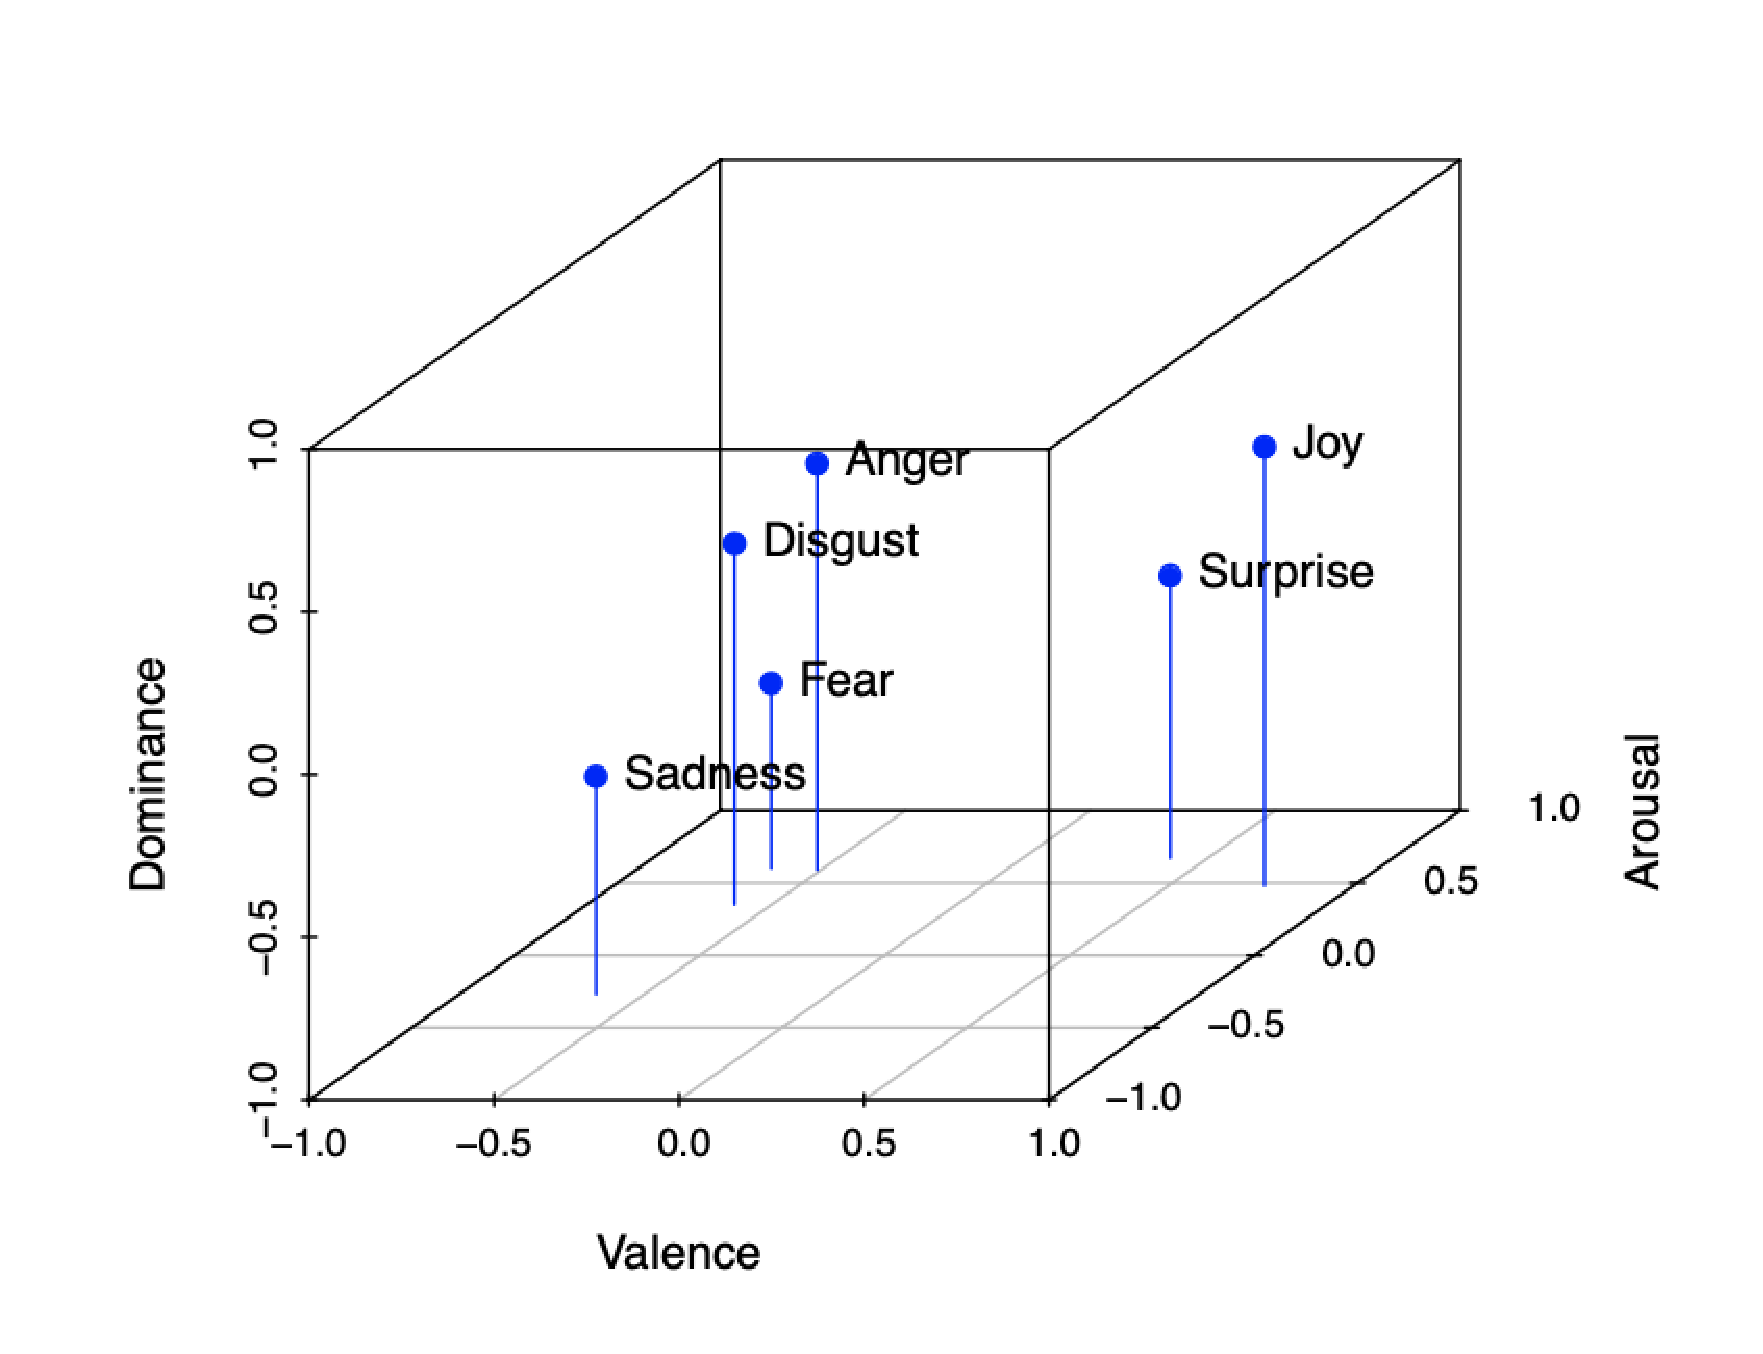
\includegraphics[height=4cm,width=6cm]{figures/six_emotions_vad.eps}
		\caption{The emotional space spanned by the Valence-Arousal-Dominance model. }\label{fig:vad}
	\end{minipage}
\end{figure}

%%==========================================================================================
%%

\section{Related Work}

\subsection{Emotion Frameworks}
\

Two main approaches of emotion representation exist, 
namely categorical approaches and dimensional approaches.
In the categorical approach, 
emotions are represented as specific discrete categories.
 Ekman’s (1992) theory of six basic emotions 
 (joy, sadness, anger, fear, disgust, and surprise) 
 is the most well-known, 
 but also Plutchik’s (1980) wheel of emotions, 
 in which joy, sadness, anger, fear, disgust, surprise, trust, 
 and anticipation are considered most basic,
is a common framework in emotion studies. 
However, 
many other theorists provide basic emotion frameworks, 
which can count up to fourteen emotion categories 
(Izard 1971; Roseman 1984).

In dimensional models, 
emotions are represented as a point in a multidimensional space. 
According to Mehrabian and Russell (1974), 
every emotional state can be described by 
scores on the dimensions valence (unhappiness-happiness), 
arousal (calmness-excitement) and dominance (submission-dominance),
known as the VAD-model. 
However, 
in later work Russell (1980) argued that 
the two dimensions valence and arousal suffice 
for describing emotional states, 
whereas Fontaine et al. (2007) suggest adding a fourth dimension: 
unpredictability.


%%==========================================================================================
%%

\subsection{Label Distribution Learning}
\

In the LDL framework, 
each instance is labeled by a real-valued vector
The goal of LDL is to 
predict multiple real-valued description degrees of the labels.
The instance variable is denoted by $ x $ , 
the particular \textit{i}-th instant is denoted by $ x_{i} $, 
the label variable is denoted by $ y $,
the particular \textit{j}-th label value is denoted by $ y_{j} $, 
the description degree of $ y $ to $ x $ is denoted by $ d ^ y_{x} $, 
and the label distribution of $ x $ is denoted by 
$  D_{i}  = \{ d^{{y_{1}} }_{ x_{i} }, d^{{y_{2}} }_{ x_{i} },...,d^{{y_{c}} }_{ x_{i} } \} $,
where $ c $ is the number of possible label values
and $ \sum_{y}  d^y_{x} = 1 $.
$ d^y_{x}  $ can be represented by 
the form of conditional probability, i.e., 
$ d^y_{x} =  P (y|x)$. 

Suppose $ p(y|x) $  is a parametric model
$ p(y|x;{\theta}) $, 
where $ \theta $ is the parameter vector. 
Given the training set $ S $, 
the goal of LDL is to find the $ /theta $ that 
can generate a distribution similar to $ D_{i} $
given the instance $ x_{i} $.
As for the Kullback-Leibler divergence,

\begin{equation}\label{eq:kl_divergence}
\theta^{\ast} =
\mathop{\arg\min}\limits_{\theta}
\sum\limits_{i}
\sum\limits_{j}
(d^{y_{j}}_{ x_{ i } }
\ln \dfrac{ d^{y_{j}}_{ x_{ i } } }{ p( y_{ j } | x_{ i } ;{\theta}) })
\end{equation}

Assumes the parametric model 
$ p(y|x;{\theta}) $ 
to be the maximum entropy model,	

\begin{equation}\label{eq:max_entropy}
	p(y|x;{\theta}) = \dfrac{1}{Z}
	\exp ( \sum\limits_{k}
	{\theta}_{y,k} 
	g_{k}( \textbf{x})  )
\end{equation}

where $ Z = \sum _{y}
\sum_{k}  {\theta}_{y,k}  g_{k}( \textbf{x}) $
is a normalization factor,
$ {\theta}_{y,k} $ is an element in \textbf {$\theta$} ,
and $ g_{k}( \textbf{x}) $ is the \textit{k}-th feature of\textbf{ x}.
Use a strategy similar to Improved Iterative Scaling (IIS) 
to find the best answer.

%%==========================================================================================
%%
%\section{Preliminaries} \label{sec-preliminaries}

\section{Data Set}

Emobank corpus is composed of 
several categories of 
the Manually Annotated Sub-Corpus of the American National Corpus 
and the corpus of SemEval-2007 Task 14 Affective Text. 
MASC is already annotated on various linguistic levels. 
SE07, on the other hand, bears annotations according to 
Ekman’s six Basic Emotion on a [0,100] scale, respectively. 
This collection of raw data comprises 10,548 sentences see in ~\Cref{tbl:emobank}.

Use the subset MASC corpus to train the DEDL model.
Then use this model to predict the scores of 
Valence, Arousal and Dominance dimensional emotion
for the sentences in the SE07 corpus.
Organize these data into two new data sets:

\begin{description}
	\item [DATA\_1] Predicted VAD is the features and 
	the emotion categories corresponding to 
	the max scales of the sentences in SE07.
	\item [DATA\_2] Annotated VAD is the features and 
	the emotion categories corresponding to 
	the max scales of the sentences in SE07.
\end{description}

\begin{table}[htbp]  \centering
	\caption{Genre distribution of the raw and filtered
		EMOBANK corpus.}
	\label{tbl:emobank}
	\begin{tabular}{cccc}
		\toprule
		Corpus & Domain  & Raw & Filtered  \\
		\midrule
		SE07 &  news headlines &  1250 &  1192 \\
		\hline
		\multirow{6}{*}{MASC} &  blogs&  1378&  1336\\
		&  essays &  1196 &  1135 \\
		&  fiction &  2893 &  2753 \\
		&  letters &  1479 &  1413 \\
		& newspapers & 1381 & 1314 \\
		& traval guides & 971 & 919 \\
		\bottomrule
	\end{tabular}
\end{table}

%%==========================================================================================
%%

\section{Method} \label{sec-method}

\subsection{Method One}
\

One sentence contain different scores of 
three dimensional emotions. 
We use $ d^y_{x} $ to indicate the intensity of 
dimensional emotion $ y $ for sentence $ x $, 
where $ x \in \chi  $ and $ y \in Y $.
The dimensional emotion intensity is needed to
meet the conditions that
$ d^y_{x} \in [0,1] $ and $\sum_{y}  d^y_{x} = 1$.
Note that $ d^y_{x} $ denotes the proportion that 
$ y $ accounts for in a valence, 
arousal  and dominance dimensional emotion distribution
of $ x $.

The training set is $ S = \{ ( x_{i} , D_{i} )  \}^{n}_{i=1} $,
where $ x_{i} \in \chi $ is a sentence embedding and
$ D_{I} = \{d^{y_{1}}_{x_{i}},  d^{y_{2}}_{x_{i}}, ... , d^{y_{c}}_{x_{i}}\} $
is the valence, arousal  and dominance dimensional emotion distribution.
The goal of DEDL is to 
learn a  conditional probability mass function $ p(y|x) $.
Assuming that $ p(y|x) $
is a parametric model $ p(y|x;{\theta}) $,
where $ \theta $ is model parameter.

Use the Kullback-Leibler divergence	as 
the distance measure,
the best parameter vector $ \theta^{\ast} $ is determined by
~\Cref{eq:kl_divergence}.

And for this problem,
the label distribution set $ D_{i} $ is that
$ D_{I} = \{d^{y_{v}}_{x_{i}},  d^{y_{a}}_{x_{i}}, d^{y_{d}}_{x_{i}}, d^{y_{n}}_{x_{i}}\} $,
where
$ d^{y_{v}}_{x_{i}} = \dfrac{score^{v}_{x_{i}}}{15} $,
$ d^{y_{v}}_{x_{i}} = \dfrac{score^{v}_{x_{i}}}{15} $,
$ d^{y_{v}}_{x_{i}} = \dfrac{score^{v}_{x_{i}}}{15} $,
and $ y_{n} = 1 - y_{v}  - y_{a} - y_{d} $.
The following we proof that 
LDL is valid for the valence, arousal  
and dominance dimensional emotion distribution.

Assume that 

\begin{equation}
T(\theta) =
\mathop{\arg\min}\limits_{\theta}
\sum\limits_{i}
\sum\limits_{j}
(d^{y_{j}}_{ x_{ i } }
\ln \dfrac{ d^{y_{j}}_{ x_{ i } } }{ p( y_{ j } | x_{ i } ;{\theta}) })
\end{equation}

and $ p( y_{ j } | x_{ i } ;{\theta}) $ is the~\Cref{eq:max_entropy}. 
For each step, 
it updates the current estimate of the parameters 
\textbf{$\theta$} to \textbf{ $\theta + \delta$},
where \textbf{$ \delta $} minimizes a lower bound to the change in likelihood

\begin{equation}\label{eq:update}
T(\theta + \delta) - T(\theta) =
\sum\limits_{ij} d^{y_{j}}_{ x_{ i } } ( \ln p(y_{j}|x_{i};{\theta}) - \ln p(y_{j}|x_{i};{\theta +\delta})
\end{equation}

As for the Root Mean Square Error,
the goal is 
$ \mathop{\min}\sum\limits_{ij} ( d^{y_{j}}_{ x_{ i } } -  p(y_{j}|x_{i};{\theta}))^{2}$
which is equal to

\begin{equation}\label{eq:rmse}
	R(\theta) = \mathop{\min} \sum\limits_{ij}
	|d^{y_{j}}_{ x_{ i } } -  p(y_{j}|x_{i};{\theta})|
\end{equation}

for each update,

\begin{equation}\label{eq:rmse'}
	R(\theta + \delta) - R(\theta) \leq 
	\sum\limits_{ij} |
	d^{y_{j}}_{ x_{ i } }  - 
	p(y_{j}|x_{i};{\theta + \delta}) - 
	(d^{y_{j}}_{ x_{ i } }  - 
	p(y_{j}|x_{i};{\theta})) | =
	\sum\limits_{ij}
	|  \ln p(y_{j}|x_{i};{\theta}) - \ln p(y_{j}|x_{i};{\theta +\delta} |
\end{equation}

From the ˜\Cref{eq:update} and ˜\Cref{eq:rmse'}, 
we can find that the goals of EDLD and  RMSE
when the $ \theta $ updates are the same.
So the EDLD is valid.
   
%%==========================================================================================
%%

\subsection{Method Two}

\subsubsection{TextCNN}
\

TextCNN mainly uses 
a one-dimensional convolutional layer and 
max-over-time pooling layer. 
Suppose the input text sequence consists of $ n $ words, 
and each word is 
represented by a $ d $-dimension word vector. 
Then the input example has a width of $ n $,
a height of  1, and $ d $ input channels. 
The calculation of textCNN can 
be mainly divided into the following steps:

\begin{itemize}
	\item 
	Define multiple one-dimensional convolution kernels 
	and use them to 
	perform convolution calculations on the inputs. 
	Convolution kernels with different widths may 
	capture the correlation of different numbers of adjacent words.
	\item 
	Perform max-over-time pooling 
	on all output channels, 
	and then concatenate the pooling output values of 
	these channels in a vector.
	\item 
	The concatenated vector is 
	transformed into the output for 
	each category through the fully connected layer. 
	A dropout layer can be used in 
	this step to deal with overfitting.
\end{itemize}

\Cref{fig:cnn}gives an example to illustrate the textCNN.
The input here is a sentence with 11 words, 
with each word represented by 
a 6-dimensional word vector. 
Therefore, 
the input sequence has 
a width of 11 and 6 input channels. 
We assume there are 
two one-dimensional convolution kernels 
with widths of 2 and 4, 
and 4 and 5 output channels, 
respectively. 
Therefore, 
after one-dimensional convolution calculation, 
the width of the four output channels is  $ 11-2+1=10 $,
while the width of the other five channels is  $ 11-4+1=8 $. 
Even though the width of each channel is different, 
we can still perform max-over-time pooling for 
each channel and concatenate the pooling outputs of 
the 9 channels into a 9-dimensional vector. 
Finally, 
we use a fully connected layer to 
transform the 9-dimensional vector 
into a 2-dimensional output: 
positive sentiment and negative sentiment predictions.

\begin{figure}[htbp]
	\centering
	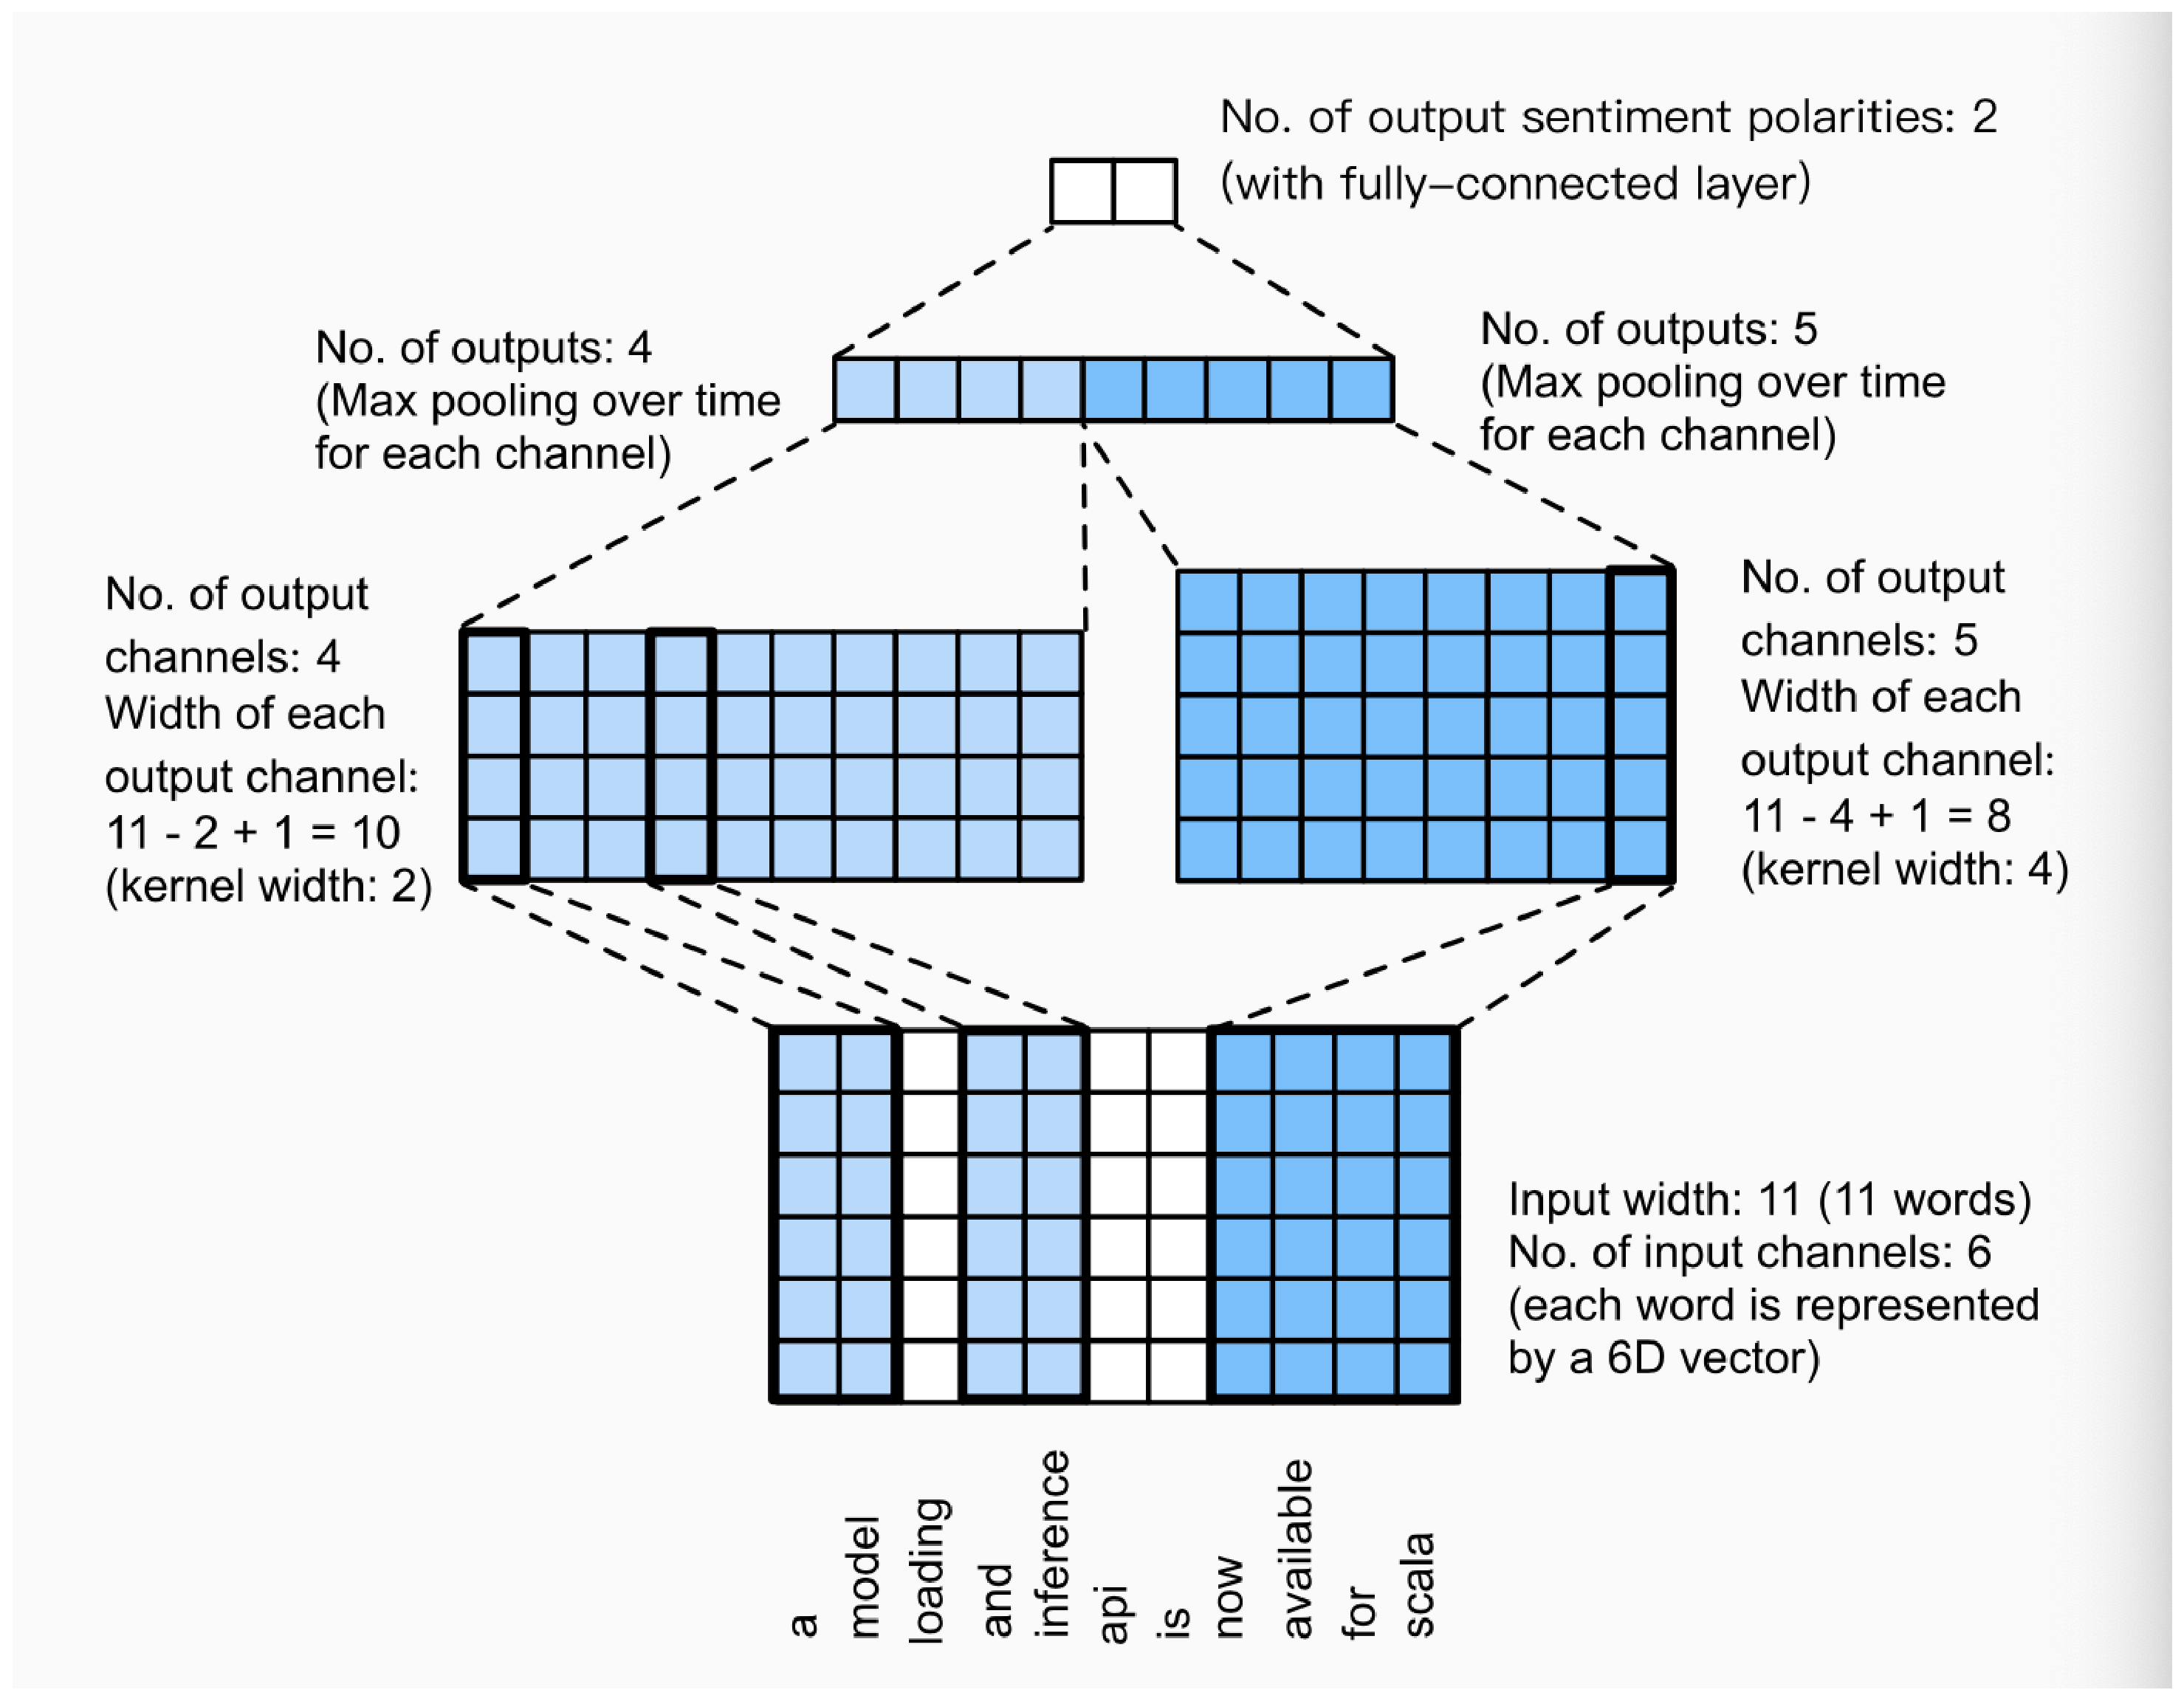
\includegraphics[height=5cm,width=8cm]{figures/textCNN_en.eps}
	\caption{The emotional space spanned by the Valence-Arousal model}\label{fig:cnn}
\end{figure}

%%==========================================================================================
%%
\subsubsection{LSTM}
\

The challenge to 
address long-term information preservation 
and short-term input skipping 
in latent variable models 
has existed for a long time. 
One of the earliest approaches to 
address this was the LSTM. 
It shares many of 
the properties of the Gated Recurrent Unit. 

Arguably it is inspired by 
logic gates of a computer. 
To control a memory cell 
we need a number of gates. 
One gate is needed to 
read out the entries from the cell 
(as opposed to reading any other cell). 
We will refer to this as the output gate. 
A second gate is needed to 
decide when to read data into the cell. 
We refer to this as the input gate. 
Last, 
we need a mechanism to 
reset the contents of the cell, 
governed by a forget gate. 
The motivation for 
such a design is the same as before, 
namely to be able to decide 
when to remember and 
when to ignore inputs 
in the latent state 
via a dedicated mechanism. 
The structure of LSTM is showed in \Cref{fig:lstm}.

In this model, 
each word first obtains a feature vector 
from the embedding layer. 
Then, 
we further encode the feature sequence using 
a bidirectional recurrent neural network to 
obtain sequence information. 
Finally, 
we transform 
the encoded sequence information to 
output through the fully connected layer. 
Specifically, 
we can concatenate hidden states of 
bidirectional long-short term memory 
in the initial timestep and final timestep 
and pass it to the output layer classification 
as encoded feature sequence information. 
In the BiRNN class implemented below, 
the Embedding instance is 
the embedding layer, 
the LSTM instance is 
the hidden layer for sequence encoding, 
and the ,Linear instance is 
the output layer for generated classification results.

\begin{figure}[htbp]
	\centering
	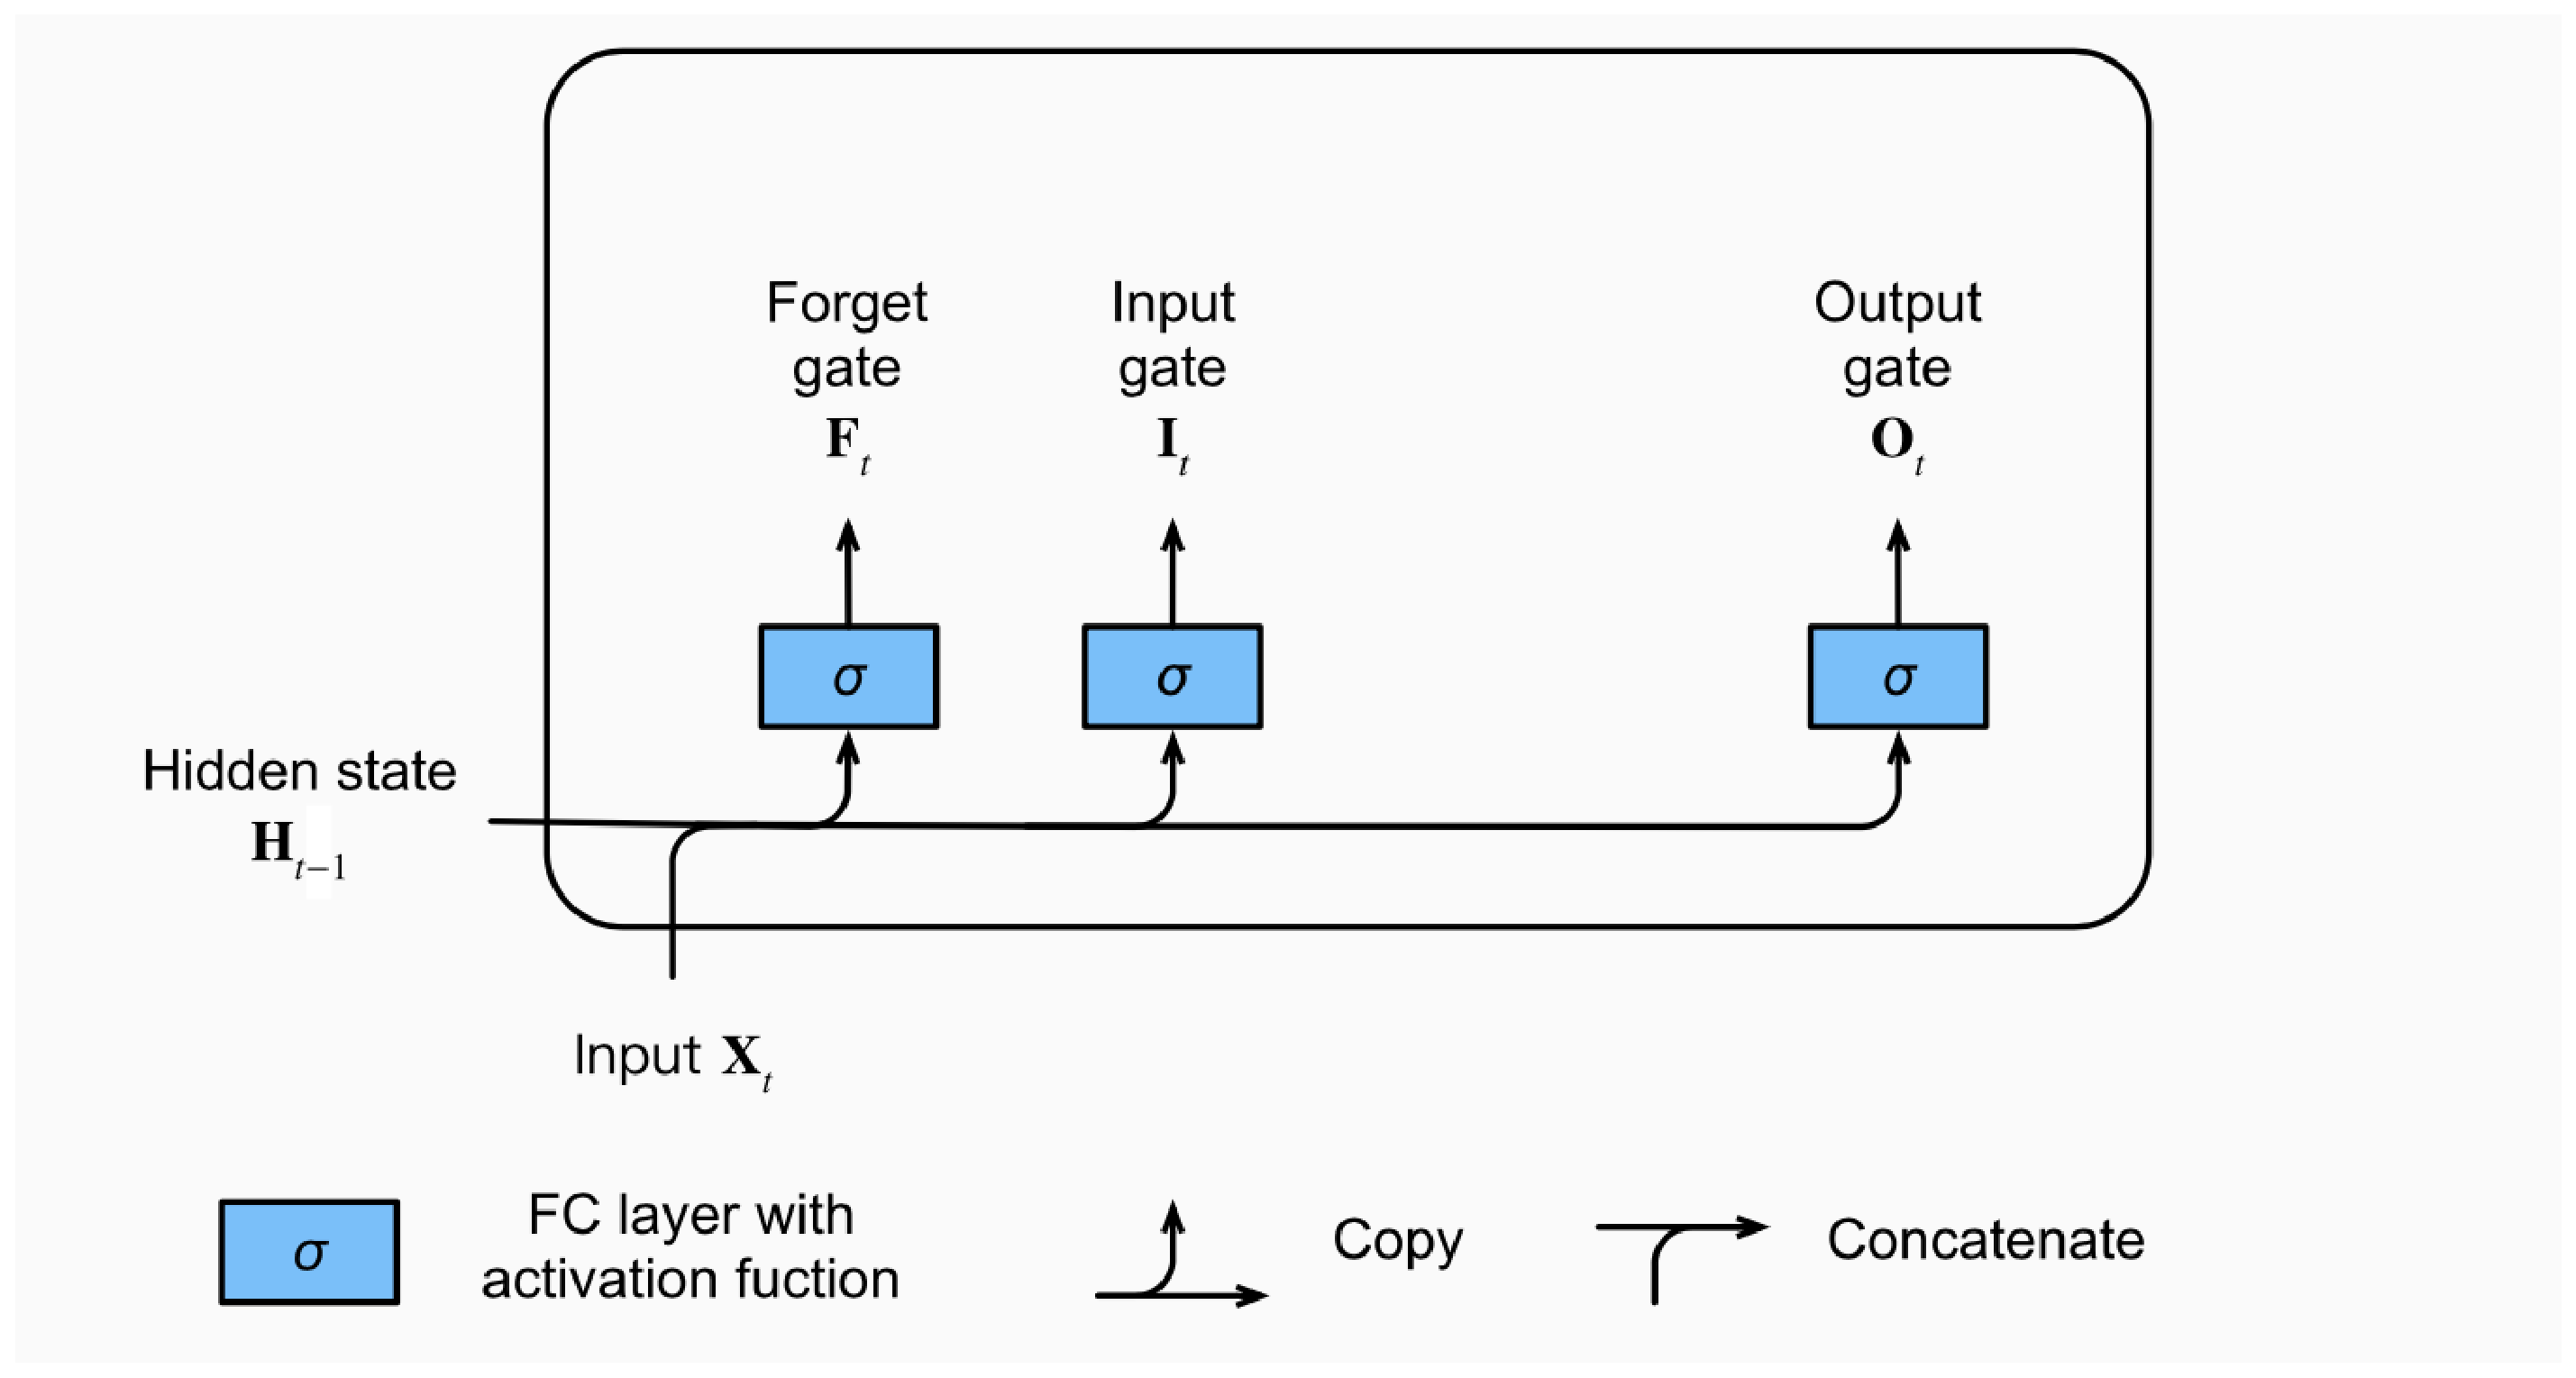
\includegraphics[height=4cm,width=7cm]{figures/lstm_en.eps}
	\caption{The emotional space spanned by the Valence-Arousal model}\label{fig:lstm}
\end{figure}


%%==========================================================================================
%%

\section{Experiment and Analysis} \label{sec-experiment}

\subsection{Experiment}

\subsubsection{Experiment One}
\

\begin{itemize}
	\item
	Data Processing
	
	\begin{itemize}
		\item 
		Use Bert to train the sentence encoding/embedding
		of Emobank corpus, that is the feature vectors $ x_{i} $
		\item 
		Transform the scores of Valence, Arousal and Dominance 
		dimensional emotion into 
		the label distribution 
		$ D_{i} = \{d^{y_{v}}_{x_{i}},  d^{y_{a}}_{x_{i}}, d^{y_{d}}_{x_{i}}, d^{y_{n}}_{x_{i}}\} $,
	\end{itemize}
	
	\item 
	Predict the scores of 
	Valence, Arousal and Dominance dimensional emotion
	through the EDLD
	for the sentences in the SE07 corpus.
	
	\item 
	New Data Set
	
	\begin{itemize}
		\item 
		DATASET_1 : predicted VAD is the features and 
		the emotion categories corresponding to 
		the max scales of the sentences in SE07.
		\item 
		DATASET_2 : Annotated VAD is the features and 
		the emotion categories corresponding to 
		the max scales of the sentences in SE07.
	\end{itemize}
	
	\item 
	Algorithm
	
	\begin{itemize}
		\item DecisionTree, KNeighbors, LogisticRegression and so on.
		
	\end{itemize}
\end{itemize}


%%==========================================================================================
%%

\subsubsection{Experiment Two}
\

\begin{itemize}
	
	\item 
	Load data : The function in codes 
	reads the dataset into a list of sentences, 
	each sentence is a string. 
	Here we ignore punctuation and capitalization.
	\item 
	Text Preprocessing
	
	\begin{itemize}
		\item 
		Tokenization : For each sentence, 
		we split it into a list of tokens. 
		A token is a data point the model will train and predict. 
		The function in code supports 
		splitting a sentence into words or characters, 
		and returns a list of split strings.
		\item 
		Vocabulary : The vocabulary is used to 
		map string tokens into numerical indices starting from 0. 
		To do so, 
		first count the unique tokens in all documents, 
		called corpus, 
		and then assign a numerical index to 
		each unique token according to its frequency. 
		Rarely appeared tokens are 
		often removed to reduce the complexity. 
		A token does not exist in corpus or 
		has been removed is mapped into 
		a special unknown (“unk”) token. 
		\item 
		Data iterator
	\end{itemize}
	
	\item 
	Using a TextCNN or LSTM Model
	
	\item 
	Loading Pre-trained Word Vectors :
	Because the training dataset for 
	sentiment classification is not very large, 
	in order to deal with overfitting, 
	we will directly use word vectors pre-trained on 
	a larger corpus as the feature vectors of all words. 
	Here, we load a 300-dimensional GloVe word vector
	 for each word in the dictionary vocab.
	
	\item 
	Training and Evaluating the Model
	
\end{itemize}

%%==========================================================================================
%%
\subsection{Analysis}
\

From the table below
shows the result of base models
on DATA\_1 and DATA\_2.

\begin{table} [htbp] \centering
  \caption{Precision Comparison on Event Detection Methods}
  \label{tbl:overall-experiments}
  \begin{tabular}{cccccc}
\toprule
 & RandomForest  & Bagging & Boosting & KNN & SVC\\
\midrule
DATA\_1&  0.32 &  0.30 &  0.30 & 0.31 & 0.33\\
DATA\_2 &  0.35 &  0.34 &  0.34 & 0.30 & 0.34\\
\bottomrule
\end{tabular}
\end{table}


%%==========================================================================================
%%

\section{Conclusions} \label{sec-conclusions}



\section*{Acknowledgment}

\lipsum[1]


The authors would like to thank \ldots

